%% Korean draft translated from main.tex on 2026-06-13
%% for the International Conference ICCAS 2026

\documentclass[10pt,twocolumn]{ICCAS}

\usepackage{kotex}
\usepackage{amsmath,amssymb,amsfonts}
\usepackage{graphicx}
\usepackage{booktabs}
\usepackage{diagbox}

\linespread{0.97}

\renewcommand{\topfraction}{0.95}
\renewcommand{\bottomfraction}{0.95}
\renewcommand{\textfraction}{0.05}
\renewcommand{\floatpagefraction}{0.95}

\begin{document}
\raggedbottom

\title{3D Gaussian Splatting과 RL 유도 흔들림을 이용한 사족 보행 로봇 비전 자율주행의 지각-동역학 간극 완화 파이프라인}

\author{이민석${}^{1}$, 한성유${}^{1}$, 문희재${}^{1}$, 황성수${}^{1*}$ }

\affils{ ${}^{1}$한동대학교 AI융합교육원, 전산전자공학부, \\
경상북도 포항시 북구 흥해읍 한동로 558, 대한민국 \\
(\{glen, tjsrb439, 22000249\}@handong.ac.kr, sshwang@handong.edu) {\small${}^{*}$ 교신저자}}

\abstract{
    실제 환경에서 물리적인 사족 보행 로봇에 자율 비전 주행 시스템을 직접 검증하고 배포하는 것은 지각 수준의 sim-to-real 간극, 즉 합성 환경의 시각적 사실성 부족, 그리고 보행으로 인해 발생하는 카메라 흔들림(ego-motion jitter)이라는 심각한 문제를 가진다. 이러한 진동은 RGB-D 특징점 추적과 깊이 일관성을 저하시킨다. 본 논문은 이러한 문제를 안전하고 효율적으로 해결하기 위해, 가상 검증과 직접적인 파라미터 최적화를 가능하게 하는 지각 및 동역학 간극 완화 파이프라인을 제안한다. 가상 sandbox 단계에서는 실제 캠퍼스 복도에 대한 고충실도 3D Gaussian Splatting(3DGS) 디지털 트윈을 재구성하고, 시뮬레이션에서 강화학습(RL) 보행 정책을 활용하여 보행 동역학을 능동적으로 모사함으로써 대표적인 카메라 bobbing noise를 생성한다. 이렇게 동기화된 시각 및 동역학 교란 조건에서 RTAB-Map visual SLAM과 Nav2 스택의 파라미터를 사전 튜닝하고 최적화한다. 배포 단계에서는 RL 정책을 우회하고, custom ROS 2 bridge를 통해 주행 속도 명령을 물리 로봇의 내장 Sport API로 직접 전달한다. 실제 복도 환경에서의 실험 결과는 시뮬레이션된 RL 유도 흔들림 조건에서 최적화된 파라미터가 물리 플랫폼으로 직접 전이되어, 실제 환경에서의 파라미터 재조정 없이 안정적인 비전 기반 지도작성과 자율 장애물 회피를 달성함을 보인다.
}

\keywords{
    사족 보행, Visual SLAM, Sim-to-Real 파이프라인, 3D Gaussian Splatting, Ego-motion Jitter, 가상 Sandbox.
}

\maketitle

\begin{figure*}[t]
\begin{center}
\vspace{-2mm}
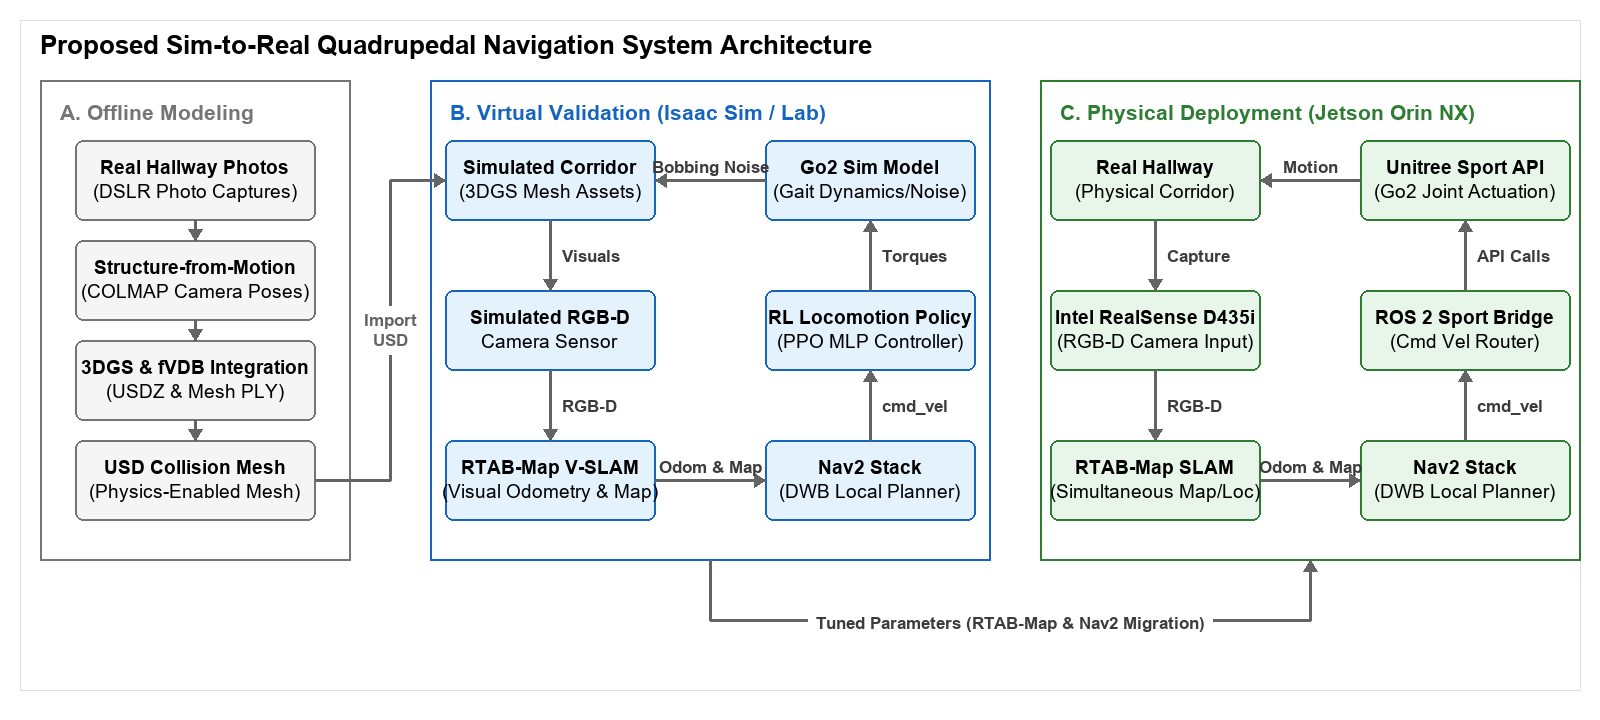
\includegraphics[width=\textwidth]{figures/fig_system_overview}
\vspace{1mm}
\caption{\label{fig_system_overview}제안하는 sim-to-real 사족 보행 로봇 주행 프레임워크의 전체 구조. (a) 가상 검증 단계에서는 고충실도 3DGS 환경을 구축하고, 상위 주행 파라미터 튜닝을 위해 카메라 bobbing noise를 모사하는 RL 보행 정책을 학습한다. (b) 물리 배포 단계에서는 Jetson Orin NX의 연산 자원을 최적화하기 위해 RL 정책을 우회하고, ROS 2 bridge를 통해 Unitree Sport API로 명령을 전달한다.}
\vspace{-3.5mm}
\end{center}
\end{figure*}

%-----------------------------------------------------------------------

\section{서론}
자율 사족 보행 로봇은 일반적인 바퀴형 시스템에 비해 험지 및 비정형 지형을 통과하는 우수한 이동성을 가지므로 많은 관심을 받아왔다. 실내 환경에서 완전한 자율 동작을 달성하기 위해서는 안정적인 보행 제어와 고충실도 동시적 위치추정 및 지도작성(SLAM)의 매끄러운 통합이 필요하다. 전통적으로 실내 주행은 Light Detection and Ranging(LiDAR) 센서에 의존해 왔다. 그러나 LiDAR는 비용이 높고 무거우며 전력 소모가 크기 때문에, 단일 경량 RGB-D 카메라를 사용하는 비전 기반 주행은 매우 매력적인 비용 효율적 대안이 된다.

그럼에도 단일 RGB-D 카메라를 사용하는 비전 기반 주행을 보행 플랫폼에 배포할 때는 두 가지 핵심적인 sim-to-real 문제가 발생한다. 첫 번째는 \textit{지각적 sim-to-real 간극}이다. 일반적인 물리 시뮬레이터는 사실적인 시각 텍스처와 깊이 충실도가 부족한 합성 환경을 생성하며, 이로 인해 특징점 기반 visual SLAM은 심각한 매칭 오류 때문에 실제 환경에서 실패할 수 있다. 두 번째는 \textit{보행으로 유도되는 ego-motion noise}(일반적으로 bobbing noise라고 부름)이다. 보행 이동은 본질적으로 주기적이고 고주파적인 카메라 진동을 발생시키며, 이는 motion blur를 일으키고 시간적 깊이 불일치(phantom obstacle)를 유발한다. 사족 보행 로봇은 매우 고가이고 정교한 플랫폼이므로, 이러한 교란을 완화하기 위한 주행 파라미터를 물리 하드웨어에서 직접 튜닝하는 것은 큰 제약을 가진다. 실제 환경 실험은 배터리 용량으로 인해 엄격한 시간 제한을 받으며, 파라미터 튜닝 중 제어 또는 지도작성 실패가 발생하면 고가의 로봇에 충돌로 인한 심각한 물리적 손상을 초래할 수 있다.

이러한 한계를 해결하기 위해 본 논문은 단일 전방 RGB-D 카메라(Intel RealSense D435i)를 사용하는 사족 보행 로봇 비전 주행을 위한 실용적인 이중 단계 간극 완화 파이프라인을 제안한다. 제안 프레임워크는 가상 공간에서의 파라미터 검증과 물리 공간에서의 시스템 배포를 분리한다. 특히 오프라인 3DGS 재구성에는 DSLR 이미지를 사용하고, 가상 카메라의 파라미터를 물리 D435i 센서와 일치시킴으로써 센서 불일치를 최소화한다. 시뮬레이션 단계에서는 3DGS를 사용하여 실내 복도의 사실적인 디지털 트윈을 재구성한다. 로봇의 독점적인 저수준 제어기를 물리 시뮬레이터에 직접 통합할 수 없기 때문에, Isaac Lab에서 model-free RL 보행 정책을 학습하여 실제 gait 특성을 모사하고 가상 환경에서 대표적인 카메라 ego-motion noise를 생성한다. 이렇게 합성된 시각 및 동역학 sandbox 안에서 RTAB-Map과 Nav2 프레임워크의 파라미터를 최적화한다. 물리 배포 단계에서는 deep neural network 정책을 우회하고, 경량 ROS 2 bridge를 통해 제조사 내장 Sport API로 주행 명령을 전달하여 엣지 컴퓨터의 자원 예산을 visual SLAM과 navigation에 집중한다.

본 연구의 기여는 다음과 같다.
\begin{enumerate}
    \setlength{\itemsep}{1pt}
    \setlength{\parskip}{0pt}
    \setlength{\parsep}{0pt}
    \item DSLR 기반 3DGS와 \textit{fVDB} 재구성을 물리 시뮬레이터에 통합하여 지각적 sim-to-real 간극을 완화하는 시스템 통합 파이프라인을 제시한다. 또한 가상 카메라 파라미터를 물리 RGB-D 카메라와 일치시킨 사실적인 시각 검증 sandbox를 구축한다.
    \item RL 보행 정책을 능동적인 카메라 jitter 생성기로 활용하여 동역학적 sim-to-real 간극을 완화하고, 가상 sandbox 안에서 사족 보행 특유의 보행 진동을 재현한다.
    \item 시뮬레이션된 시각 및 동역학 교란 조건에서 최적화한 주행 및 지도작성 파라미터가 실제 환경 재보정 없이 물리 Unitree Go2 플랫폼으로 직접 전이될 수 있음을 보임으로써 제안 파이프라인의 가능성을 입증한다.
\end{enumerate}

\section{관련 연구}
\subsection{사족 보행을 위한 강화학습}
강화학습(RL)은 보행 시스템의 제어 패러다임을 크게 발전시켰다 \cite{ref1}. Model Predictive Control(MPC) 및 Whole-Body Control(WBC)과 같은 전통적인 모델 기반 방법은 정확한 시스템 동역학과 환경 접촉 모델에 크게 의존한다. 반면 model-free RL 알고리즘은 시행착오 상호작용을 통해 사족 보행 플랫폼이 강건한 보행 정책을 획득할 수 있게 한다. NVIDIA Isaac Sim 및 Isaac Lab과 같은 고도로 병렬화된 물리 시뮬레이터의 등장은 수천 개의 동시 환경에서 deep RL 정책을 학습하는 것을 가능하게 하였다. 이러한 패러다임은 ANYmal 및 Unitree Go1/Go2와 같은 시스템에서 민첩한 보행의 실제 배포를 가능하게 하였다. 도메인 랜덤화와 커리큘럼 학습을 통해 연구자들은 동역학 간극을 줄였고, 정책이 시뮬레이션에서 물리 플랫폼으로 직접 전이될 수 있도록 하였다. 그러나 기존 보행 연구의 대부분은 gait 안정성과 외란 거부에 주로 초점을 맞추었으며, 고수준 비전 주행 통합과 센서 노이즈 특성은 충분히 다루지 않았다.

\subsection{Visual SLAM 및 자율주행 통합}
이동 로봇 주행은 높은 공간 정확도와 넓은 시야각을 가진 Light Detection and Ranging(LiDAR) 센서에 전통적으로 의존해 왔다. 그러나 LiDAR는 비용이 높고 무거우며 전력 소모가 커서, payload와 전력에 제약이 있는 사족 보행 로봇에는 적합성이 낮다. RGB-D 카메라를 활용한 Visual SLAM(VSLAM)은 가볍고 비용 효율적인 대안을 제공한다. 최신 visual SLAM 프레임워크 중 Real-Time Appearance-Based Mapping(RTAB-Map) \cite{ref2}은 appearance 기반 loop closure detection과 pose-graph optimization을 결합하여 drift가 최소화된 trajectory 추정을 생성할 수 있어 널리 사용된다. 동시에 ROS 2 Navigation(Nav2) 프레임워크 \cite{ref3}는 경로 계획과 장애물 회피를 위한 산업 표준으로 자리 잡았다.

최근 연구들은 \mbox{VR-Robo} \cite{ref5}와 같이 보행 및 주행을 위한 사실적인 디지털 트윈을 구축하기 위해 3DGS \cite{ref4}를 활용했지만, 종종 이종 센서에 의존한다. 예를 들어 \mbox{VR-Robo}는 오프라인 3DGS 모델 구축을 위해 고급 소비자용 모바일 기기(iPad 또는 iPhone 등)로 환경 장면을 촬영하지만, 학습된 정책 배포에는 물리 사족 보행 로봇에 장착된 액션 카메라(Insta360 Ace 등)를 사용한다. 서로 다른 하드웨어 구성 간에 디지털 트윈을 배포하는 것은 렌즈 왜곡 모델의 불일치, 색상 프로파일 차이, 서로 다른 field-of-view(FOV) 경계와 같은 device-level 지각 센서 간극을 유발한다. 반면 제안 파이프라인은 오프라인 3DGS 재구성에는 고해상도 DSLR 카메라를 사용하고, Isaac Sim 내부의 가상 카메라를 물리 D435i RGB-D 카메라의 FOV 및 해상도와 일치하도록 설정한다. 이러한 파라미터 동기화는 가상 시각 피드백과 실제 환경 배포 사이의 불일치를 최소화한다.

\section{시스템 및 보행 제어}
\subsection{시스템 구조}

제안 프레임워크는 RTAB-Map Visual SLAM, Nav2 navigation stack, 그리고 이중화된 보행 제어 구조를 통합한다. 제어 구조는 가상 검증 단계에서 Deep Reinforcement Learning(DRL) 보행 정책을 사용하고, 물리 배포 단계에서는 로봇의 native 저수준 Sport API로 전환한다. 시뮬레이션 단계에서는 Isaac Sim(v5.1.0) 기반 Isaac Lab(v2.3.2)에서 Proximal Policy Optimization(PPO)으로 학습된 DRL 정책을 사용하여 대표적인 사족 보행 gait 동역학과 카메라 ego-motion(bobbing) noise를 생성한다. Nav2 local planner가 계산한 고수준 속도 명령($\mathbf{v}_{cmd} = [v_x, v_y, \omega_z]^T$)은 정책의 action space로 직접 매핑된다. 실제 환경 배포 중에는 엣지 연산 자원을 절약하기 위해 연산량이 큰 DRL 정책을 우회하고, Nav2 속도 명령을 custom ROS 2 bridge를 통해 Unitree Sport API로 직접 전달한다. 이러한 자원 효율적인 구조는 Jetson Orin NX의 연산 예산을 최적화한다. 시스템 구조는 Fig.~\ref{fig_system_overview}에 나타내었다.

\subsection{Isaac Sim에서의 보행 학습}

시뮬레이션에서 대표적인 보행 동역학을 합성하고 물리적 카메라 bobbing noise를 모사하기 위해, Isaac Sim(v5.1.0) 물리 엔진 위에 구축된 NVIDIA Isaac Lab(v2.3.2)에서 RL 정책을 학습한다. 이 정책은 동적 교란 생성기로 동작하여 보행으로 인해 발생하는 카메라 진동을 생성한다. Isaac Lab의 Procedural Terrain Generator를 사용하여 불균일 지면, 램프, 계단형 장애물을 포함하는 혼합 지형 학습 환경을 구성한다. 로봇의 통과 성공률에 비례하여 장애물 높이와 경사 각도 등 지형 난이도를 동적으로 조절하는 커리큘럼 학습을 적용한다. 정책의 강건성을 높이고 sim-to-real 동역학 간극을 줄이기 위해 다음과 같은 도메인 랜덤화를 적용한다.
\begin{itemize}
    \setlength{\itemsep}{1pt}
    \setlength{\parskip}{0pt}
    \setlength{\parsep}{0pt}
    \item 몸통 질량 랜덤화: $\Delta m \in [-1.0, +3.0]$~kg.
    \item 지면 마찰 계수: $\mu \in [0.6, 0.8]$.
    \item 외란: 로봇의 center of mass(CoM)에 가해지는 impulse force perturbation.
\end{itemize}
물리 시뮬레이션 step size는 200~Hz로 설정하고, 정책 제어 루프는 50~Hz(decimation factor 4)로 실행된다.

정책은 PyTorch 기반 \textit{skrl} 라이브러리의 PPO 구현을 사용하여 학습된다. Actor와 critic 네트워크는 모두 $[512, 256, 128]$ 은닉층과 Exponential Linear Unit(ELU) 활성화 함수를 갖는 Multilayer Perceptron(MLP)으로 구성된다. 초기 학습률은 $1.0 \times 10^{-3}$이며, 목표 임계값 $0.01$을 갖는 KL-divergence adaptive scheduler로 조절된다. 할인율은 $\gamma=0.99$, Generalized Advantage Estimator(GAE) 파라미터는 $\lambda=0.95$이다.

보상 함수는 안정적인 보행 자세를 유지하면서 속도 reference를 추종하도록 설계된다. 전체 보상 $R$은 Eq. (\ref{eq_reward})와 같이 정의된다.
\vspace{-1.5mm}
\begin{equation}
R = w_{lin} R_{lin} + w_{ang} R_{ang} + w_{air} R_{air} - \sum_{i} w_{p,i} P_{i} \label{eq_reward}
\end{equation}
\vspace{-2.5mm}
여기서 각 항은 다음과 같다.
\begin{itemize}
    \setlength{\itemsep}{1pt}
    \setlength{\parskip}{0pt}
    \setlength{\parsep}{0pt}
    \item $R_{lin} = \exp(-\|\mathbf{v}_{xy}^* - \mathbf{v}_{xy}\|_2^2 / \sigma_{lin}^2)$는 선속도 추종 보상이며, $\mathbf{v}_{xy}^*$와 $\mathbf{v}_{xy}$는 각각 목표 base 선속도와 실제 base 선속도를 나타낸다($w_{lin} = 1.5, \sigma_{lin} = 0.25$).
    \item $R_{ang} = \exp(-(\omega_{z}^* - \omega_{z})^2 / \sigma_{ang}^2)$는 각속도 추종 보상이며, $\omega_{z}^*$와 $\omega_{z}$는 각각 목표 yaw rate와 실제 yaw rate를 나타낸다($w_{ang} = 0.75, \sigma_{ang} = 0.25$).
    \item $R_{air}$는 명확하고 대칭적인 gait를 유도하기 위한 foot clearance air-time 보상이다($w_{air} = 0.25$).
    \item $P_i$는 물리 제약을 강제하는 penalty term으로, base 수직 선속도, roll/pitch 진동, nominal joint limit으로부터의 편차, 과도한 torque command, 급격한 joint acceleration, 의도하지 않은 구조적 접촉을 최소화한다($w_{p,i}$는 각 penalty weight).
\end{itemize}

\subsection{3DGS 환경 구축 및 에이전트 배포}
고충실도 가상 검증 sandbox를 구축하기 위해 물리 환경을 상호작용 가능한 시뮬레이션 asset으로 변환하는 구조화된 neural reconstruction 파이프라인을 구성한다. 먼저 DSLR 카메라를 사용하여 복도의 고해상도 이미지를 촬영한다. 이러한 DSLR 기반 촬영은 고품질 3DGS 모델링에 중요한 선명한 texture와 색상 충실도를 제공하며, 스마트폰 센서에서 발생할 수 있는 공격적인 후처리 및 압축 artifact를 피할 수 있게 한다.

이 이미지들은 COLMAP 기반 Structure-from-Motion(SfM) workflow의 입력으로 사용되어 sparse camera pose와 초기 point cloud를 계산한다. 이 pose를 기반으로 3D Gaussian Splatting(3DGS) \cite{ref4} 모델을 최적화하고, 시각 렌더링을 위한 USDZ asset과 coarse geometry를 위한 Polygon Mesh PLY 파일로 내보낸다. 사실적인 시각화와 물리 충돌 사이의 간극을 줄이기 위해 재구성된 장면을 NVIDIA의 sparse volumetric data framework인 \textit{fVDB}와 통합하며, 이는 Fig.~\ref{fig_3dgs_mesh}에 나타나 있다.

\begin{figure}[thb]
\begin{center}
\vspace{-2mm}
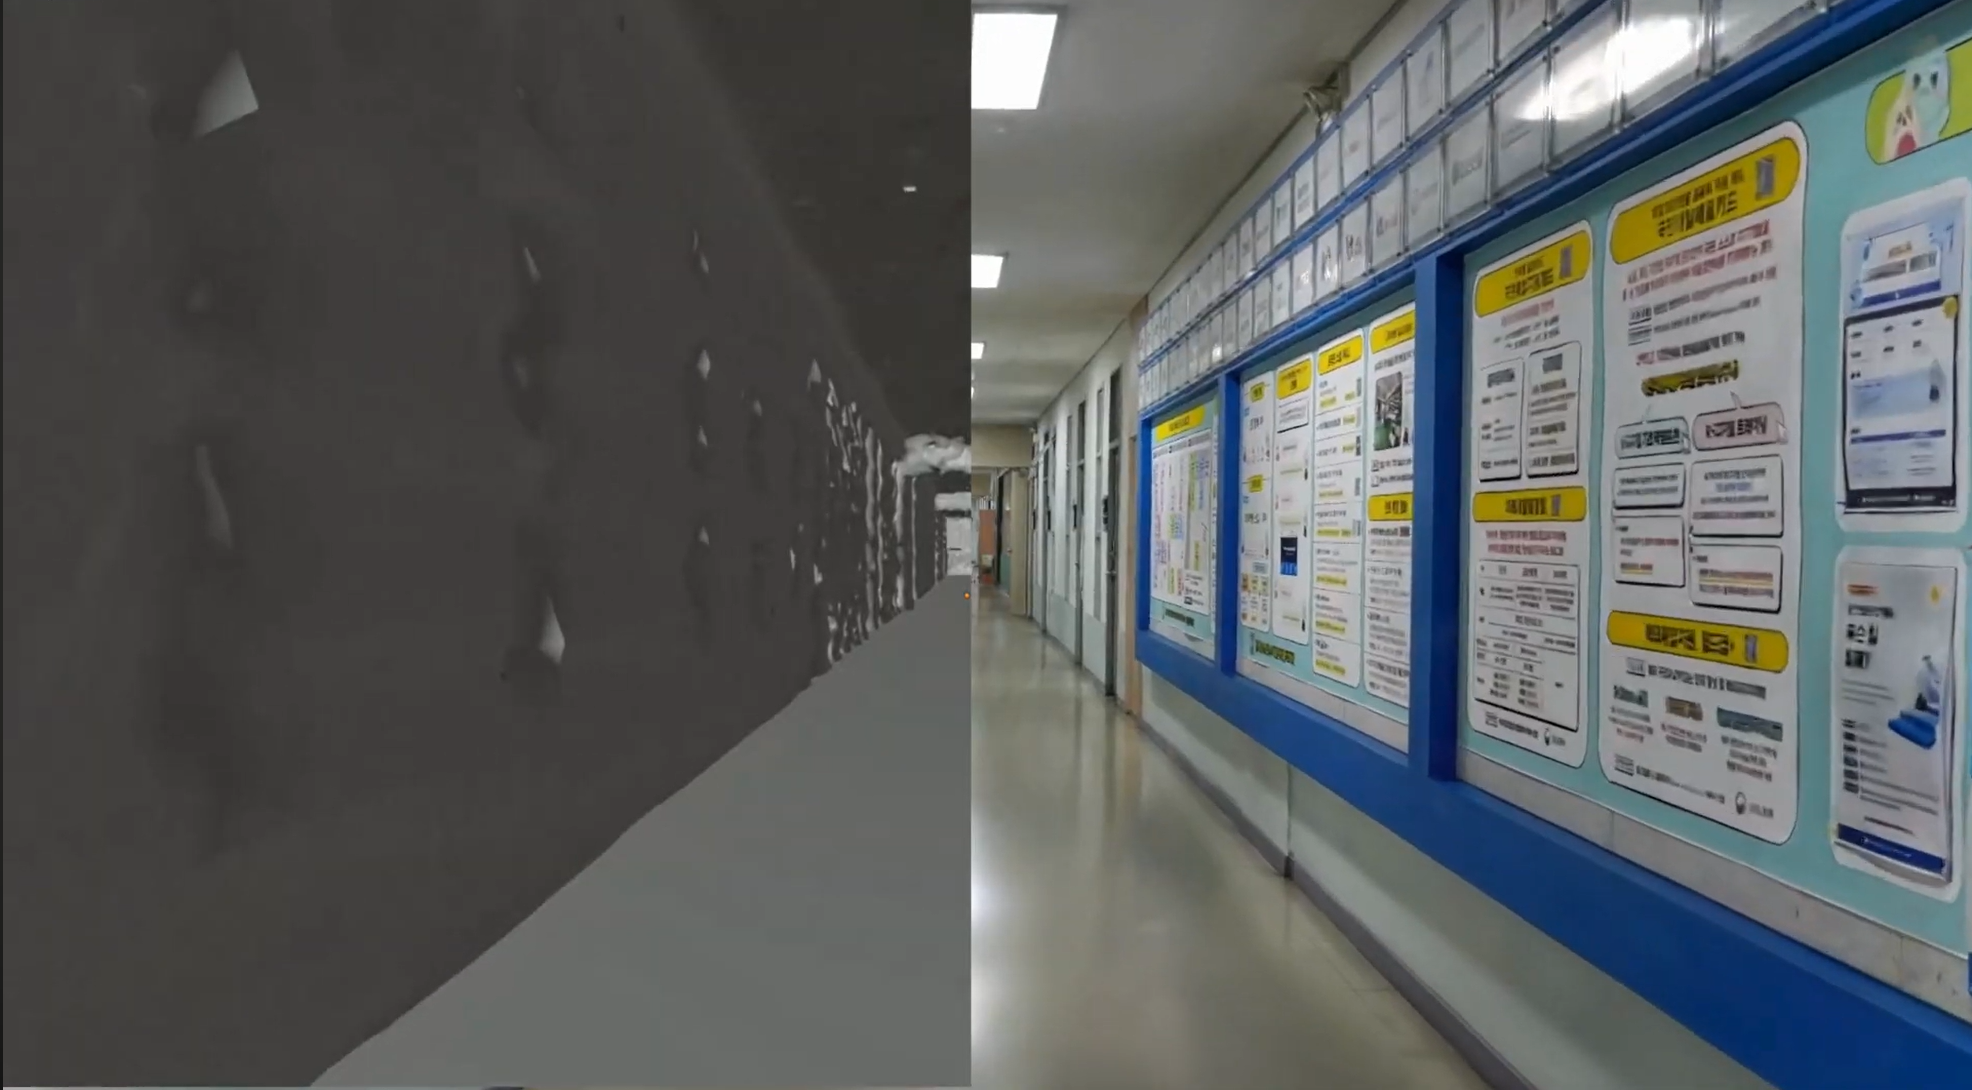
\includegraphics[width=0.8\linewidth]{figures/fig_3dgs_mesh.png}
\vspace{1mm}
\caption{\label{fig_3dgs_mesh}캠퍼스 복도에 대한 디지털 트윈 표현. 왼쪽: fVDB를 사용해 생성한 sparse volumetric collision mesh. 오른쪽: 고충실도 사실적 3DGS render.}
\vspace{-3.5mm}
\end{center}
\end{figure}

결합된 USDZ 및 mesh asset은 NVIDIA Isaac Sim(v5.1.0)으로 가져온다. 시뮬레이터 내부에서 NuRec engine은 volumetric \textit{fVDB} representation을 사용하여 고해상도 collision boundary와 동적 depth query(\textit{GS Collision / Depth})를 계산한다. 마지막으로 가상 환경과 외부 navigation stack을 연결하기 위해 ROS 2 bridge를 구축한다. 이 bridge는 가상 RGB-D camera sensor stream을 publish하고, RViz에서 로봇 상태를 시각화하며, local planner의 속도 명령을 시뮬레이션 agent로 다시 전달한다. 시뮬레이터 내부에서는 가상 카메라의 field-of-view와 해상도를 물리 Intel RealSense D435i와 일치하도록 설정한다. Isaac Sim의 virtual camera module을 사용하여 시뮬레이션 RGB-D stream이 물리 카메라의 피드백을 모사하도록 구성함으로써, 가상 환경과 실제 배포 사이의 지각적 domain shift를 최소화한다. 이후 사전 학습된 DRL 보행 정책을 추가 튜닝 없이 재구성 환경 내부의 Go2 모델에 직접 배포한다. 복잡한 기하 구조와 좁은 복도 경계에도 불구하고 정책은 강건한 gait 특성을 유지하며, 이는 도메인 랜덤화 기반 학습의 효과를 검증한다.

\section{자율주행}
\subsection{주행 시스템 구성}

제안하는 주행 시스템은 Intel RealSense D435i RGB-D 센서, RTAB-Map visual SLAM 프레임워크 \cite{ref2}, ROS 2 Nav2 stack으로 구성된 비용 효율적인 LiDAR-free 비전 주행 파이프라인이다. D435i는 Unitree Go2의 전방 torso에 견고하게 장착된다. 가상 sandbox 안에서는 시뮬레이션된 RGB-D 센서가 이에 대응되는 color 및 depth profile을 복제한다. 전체 파이프라인에 단일 RGB-D 센서를 사용하면 depth-texture 일관성도 보장된다. \mbox{VR-Robo} \cite{ref5}와 같이 순수 monocular RGB 재구성에 의존하는 프레임워크는 단색 벽이나 바닥과 같은 textureless region에서 photometric ambiguity로 인해 기하학적 hole이 발생할 수 있지만, 본 연구에서 사용하는 D435i의 active depth sensor는 강건한 metric local costmap을 투영할 수 있게 한다.

주행 workflow는 동기화된 stream들에 의해 완전히 구동된다. 먼저 RTAB-Map은 RGB stream을 처리하여 frame-to-frame Visual Odometry(VO), loop-closure detection, pose-graph optimization을 위한 visual keypoint feature(GFTT/ORB 등)를 추출한다. 이후 aligned depth stream은 이러한 feature coordinate를 사용하여 3D coordinate로 투영되고, local 3D octomap을 구성한 뒤 global path planning을 위한 2D occupancy grid map으로 투영된다. 동시에 고가의 LiDAR 장비 없이 low-latency local obstacle avoidance를 달성하기 위해 raw depth frame을 \textit{depthimage\_to\_laserscan} ROS 2 package로 pseudo-2D laser scan으로 변환한다. 이 합성 scan은 Nav2 local costmap을 채우기 위해 \textit{/scan} topic으로 publish된다. Nav2 global planner는 occupancy grid 위에서 최적 경로를 생성하고, DWB(Dynamic Window Approach B) local planner는 local costmap을 사용하여 장애물 주변으로 로봇을 안전하게 유도하는 steering command $\mathbf{v}_{cmd}$를 계산한다. 마지막으로 이 명령들은 활성화된 locomotion controller로 전달된다.

시뮬레이션 기반 검증 sandbox를 구축할 때의 핵심 기술적 문제는 물리 시뮬레이터와 표준 ROS 2 navigation stack 사이의 coordinate transform(TF) tree 불일치를 해결하는 것이다. 일반적으로 Nav2는 \textit{map} $\rightarrow$ \textit{odom} $\rightarrow$ \textit{base\_link}(또는 \textit{base}) transform chain을 기대한다. 반면 Isaac Sim은 로봇의 pose를 simulation world origin(\textit{world} frame)에 대해 정의하고 추적한다. 두 환경을 동시에 만족시키고 coordinate conflict 또는 loop를 방지하기 위해 custom static 및 dynamic transform bridge를 구현한다. 결과 TF tree는 \textit{map} $\rightarrow$ \textit{odom} $\rightarrow$ \textit{world} $\rightarrow$ \textit{base}로 구성된다. 여기서 RTAB-Map은 drift-corrected \textit{map} $\rightarrow$ \textit{odom} transform을 publish하고, Isaac Sim의 OmniGraph publisher는 odometry를 simulator global frame과 연결하며, robot state publisher가 robot physical base까지의 transform을 완성한다. 이 고유한 transform chain은 원활한 호환성을 제공하여, 표준 ROS 2 navigation 알고리즘이 코드 수정 없이 가상 sandbox 안에서 동작할 수 있게 한다.

\subsection{3DGS 환경에서의 검증}
실제 환경 배포에 앞서, 통합 navigation stack은 실제 복도와 유사한 약 80~m 길이와 2.5~m 폭의 3DGS 기반 가상 복도에서 검증되었다.

\begin{figure}[thb]
\begin{center}
\vspace{-2mm}
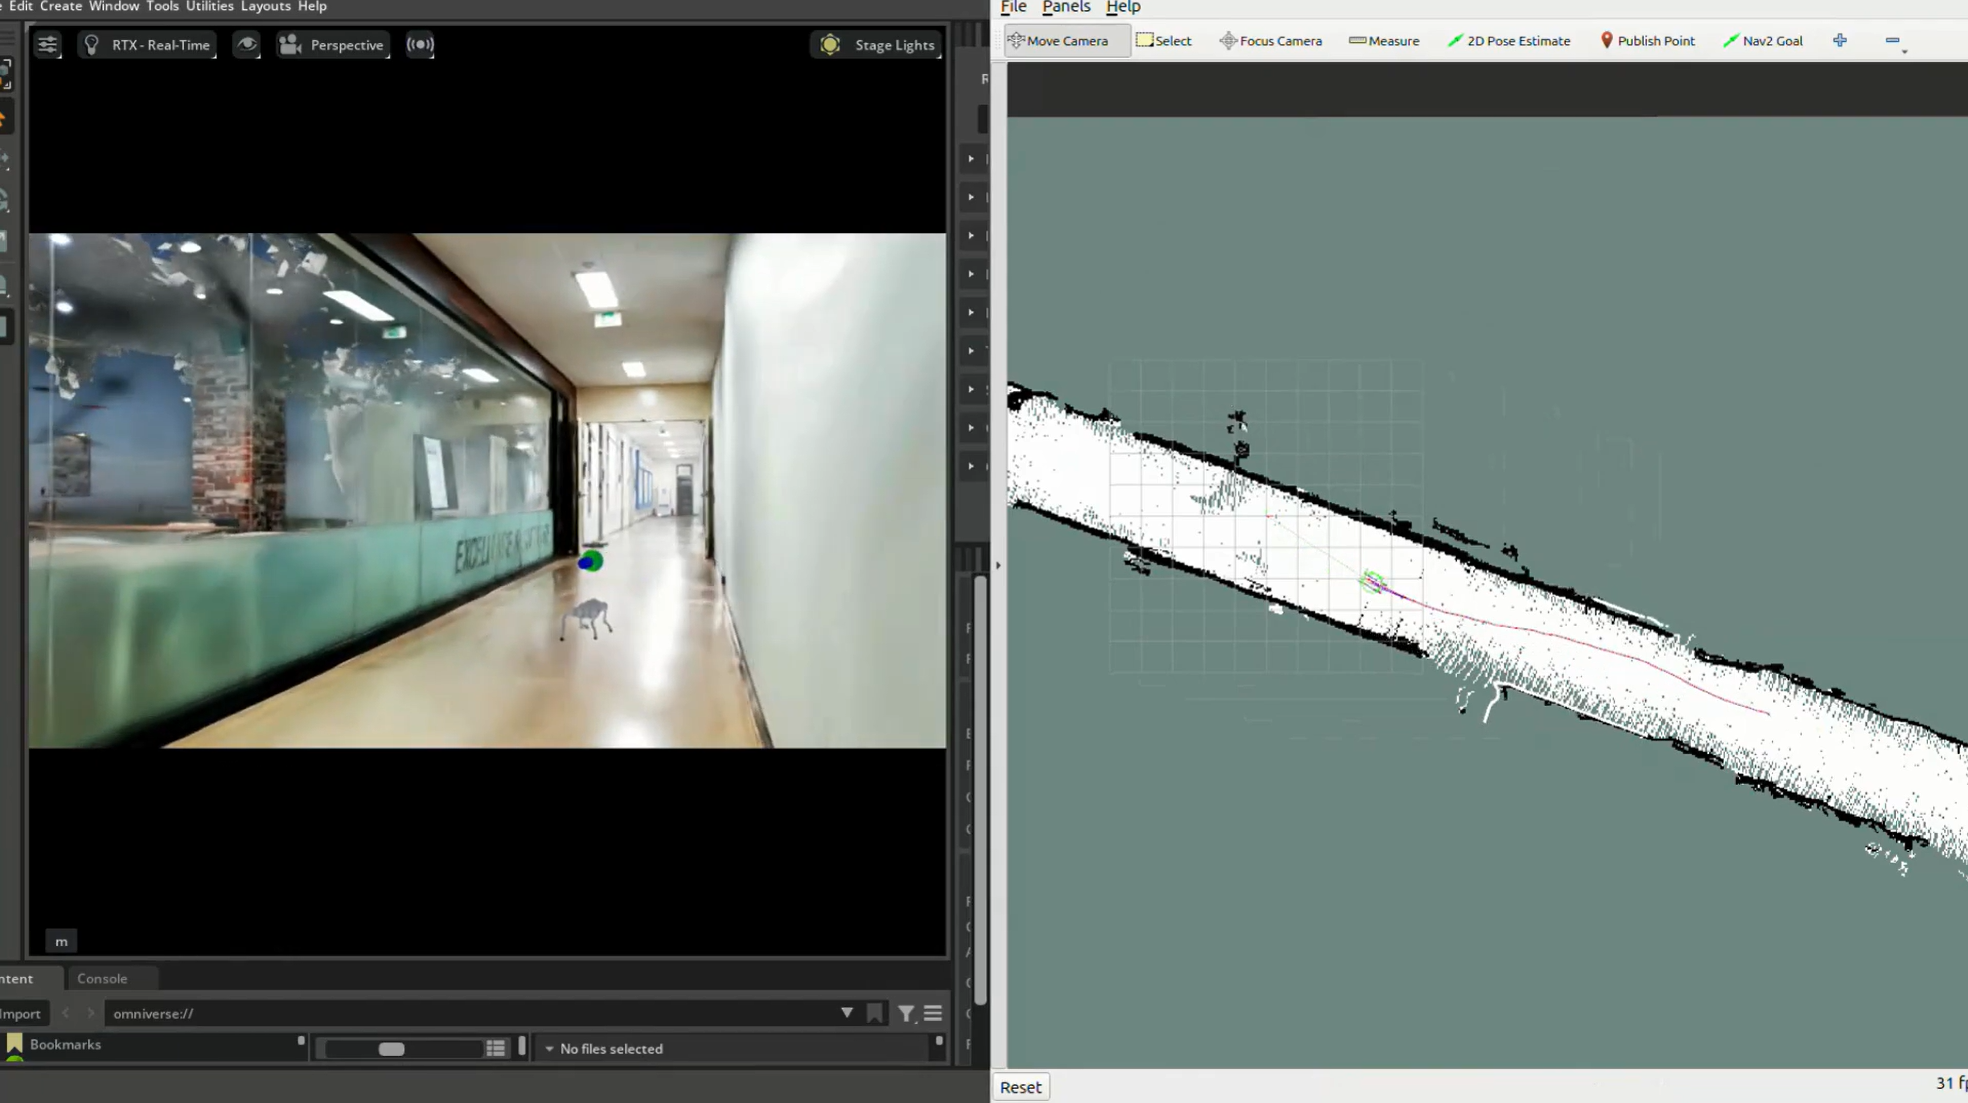
\includegraphics[width=0.8\linewidth]{figures/fig_sim_nav2.png}
\vspace{1mm}
\caption{\label{fig_sim_nav2}재구성된 가상 환경 내부에서의 자율주행 실행 장면. 왼쪽은 Isaac Sim 안의 시뮬레이션 사족 보행 로봇을, 오른쪽은 RViz에서의 경로 계획 및 costmap 동기화를 보여준다.}
\vspace{-3.5mm}
\end{center}
\end{figure}

시뮬레이션 중 정책 네트워크는 각 시간 step에서 proprioceptive 및 exteroceptive observation을 입력받는다. Proprioception은 joint position 및 velocity, base angular velocity, gravity vector projection으로 구성된다. Exteroception은 로봇 base를 중심으로 하는 가상 height-scan grid($1.6\text{ m} \times 1.0\text{ m}$, 해상도 0.1~m)를 사용하여 모사된다. Ray-casting은 재구성된 3DGS collision mesh에 대해 query를 수행하여 local elevation profile을 정책에 제공하고, 이를 통해 adaptive foot placement가 가능해진다. Reference command vector $[v_x, v_y, \omega_z]^T$는 DWB local planner가 직접 제공하며, Fig.~\ref{fig_sim_nav2}에 시각화된 것처럼 가상 환경 내부에서 충돌 없는 경로를 조정한다.

\begin{figure}[thb]
\begin{center}
\vspace{-2mm}
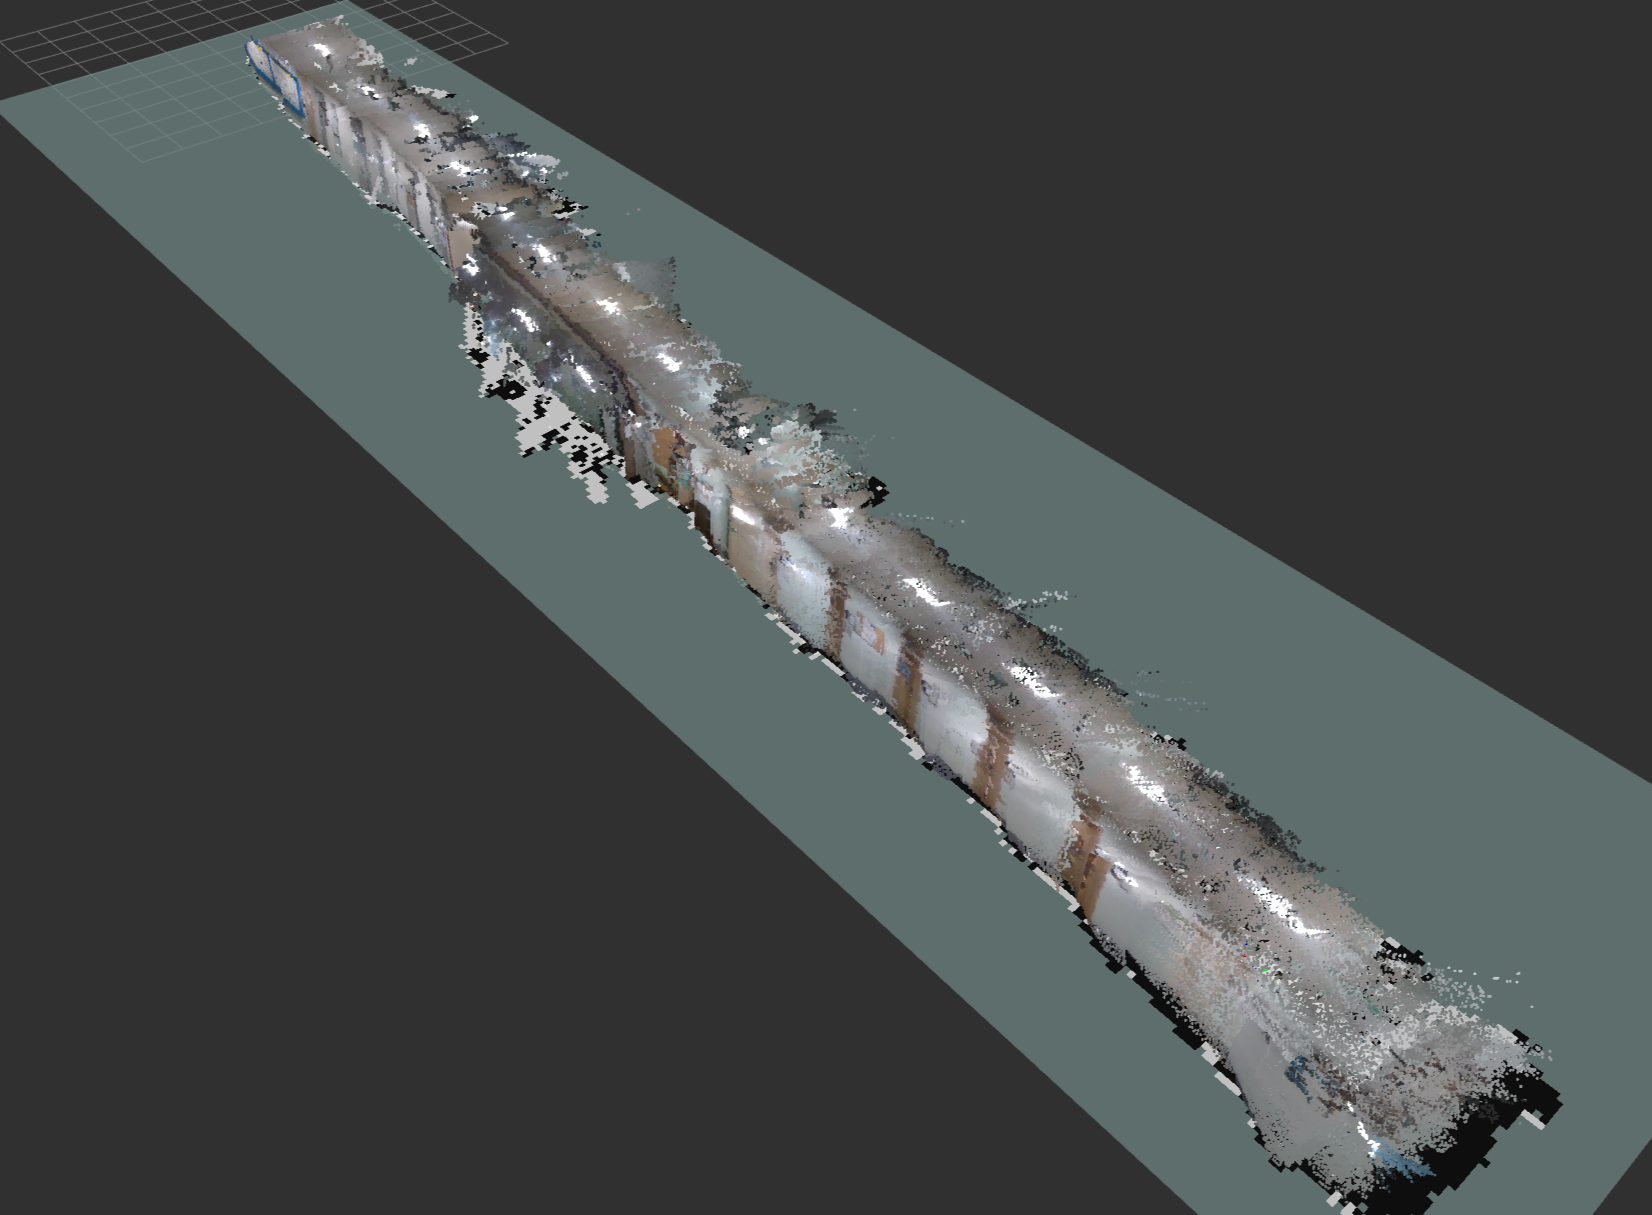
\includegraphics[width=0.55\linewidth]{figures/fig_3d_map.png}
\\
\vspace{1.5mm}
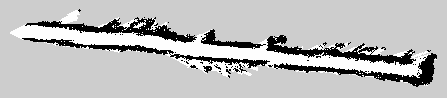
\includegraphics[width=0.55\linewidth]{figures/fig_2d_map.png}
\vspace{1.5mm}
\caption{\label{fig_sim_validation}가상 sandbox에서의 visual mapping 결과. 위: RTAB-Map으로 재구성한 3D point cloud map. 아래: 투영된 2D occupancy grid map.}
\vspace{-3.5mm}
\end{center}
\end{figure}

장애물 회피 성능을 평가하기 위해 가상 box 장애물을 복도에 전략적으로 배치하였다. Fig.~\ref{fig_sim_nav2}에 보인 것처럼 local planner는 장애물 주변으로 trajectory를 동적으로 재계산하였고, RL 보행 정책은 보행 패턴을 조정하여 충돌 없이 우회 경로를 통과하였다. 그 결과 생성된 3D point cloud map과 투영된 2D occupancy grid map은 Fig.~\ref{fig_sim_validation}에 나타내었다.
\begin{figure}[!t]
\begin{center}
\vspace{-2mm}
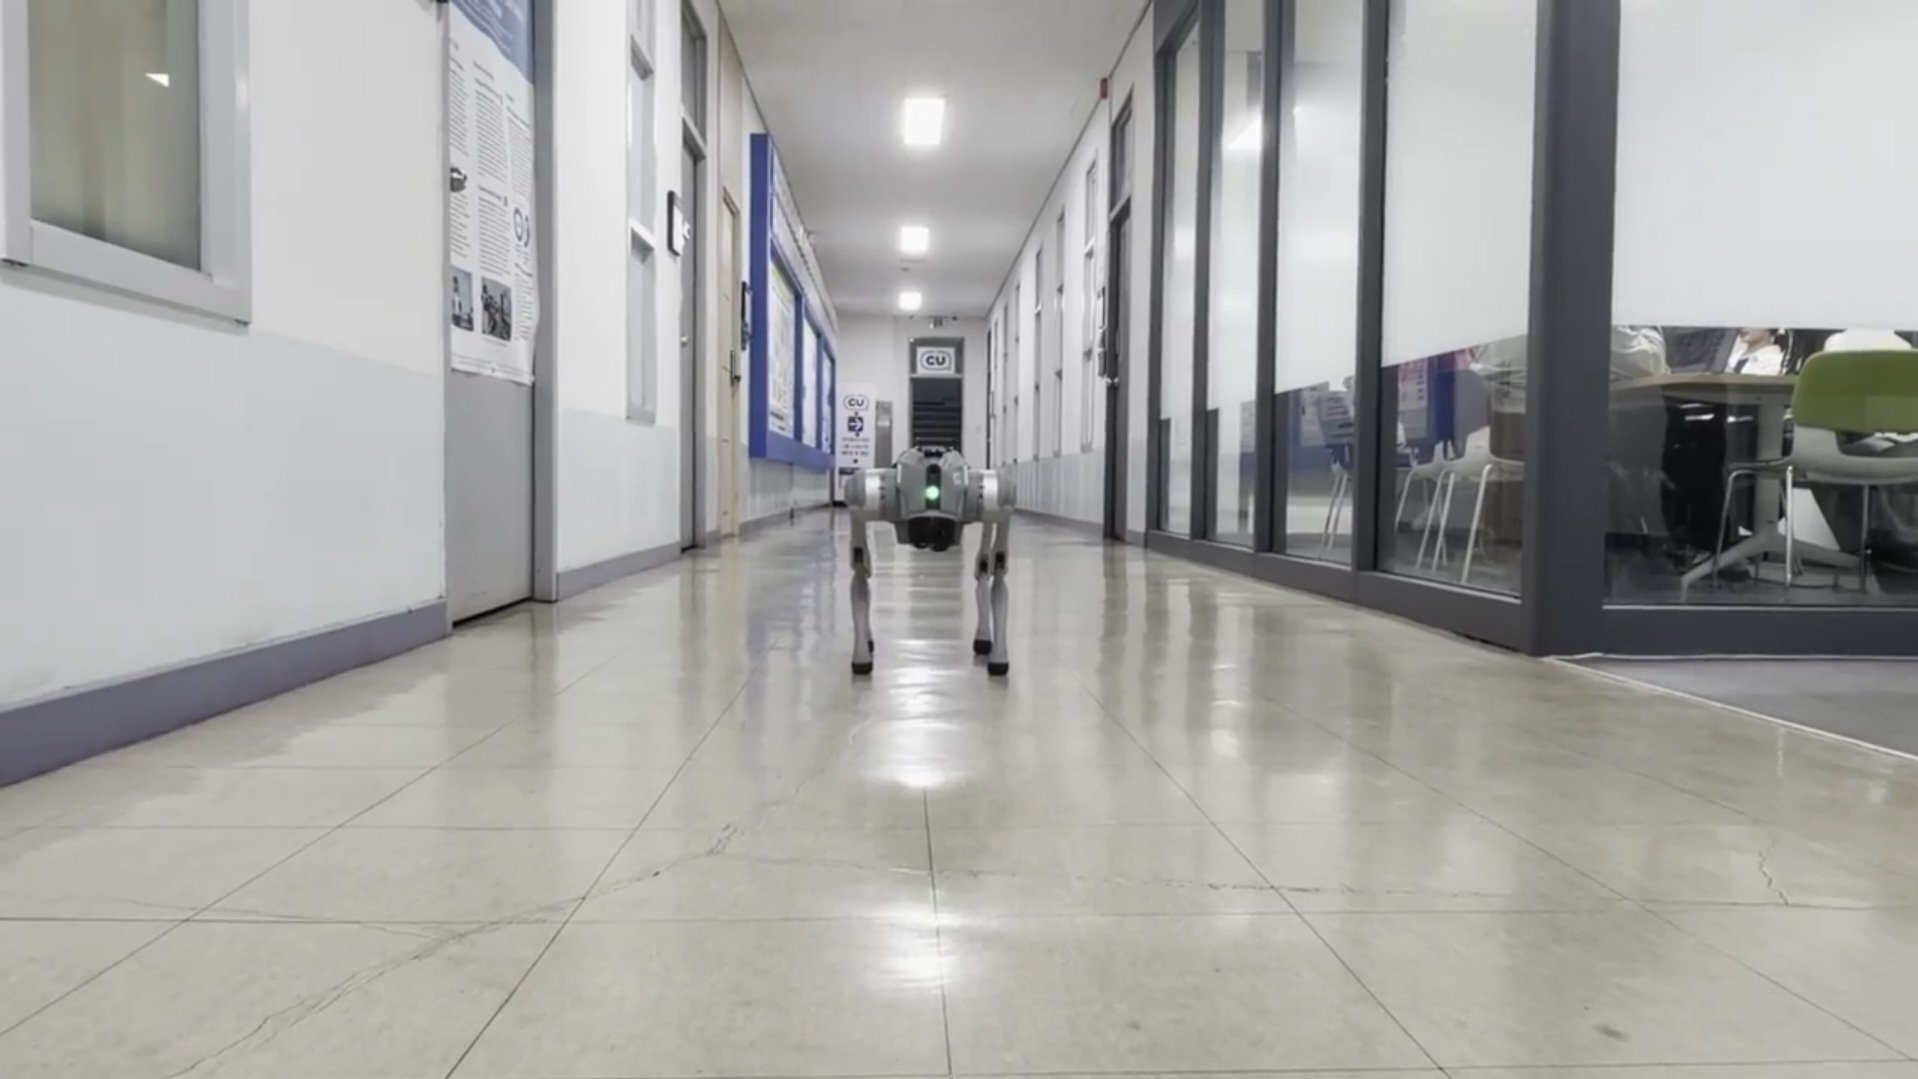
\includegraphics[width=0.8\linewidth]{figures/fig_real_robot.jpg}
\vspace{1mm}
\caption{\label{fig_real_deployment}실제 환경 실험 구성. Unitree Go2 로봇에는 Intel RealSense D435i와 Jetson Orin NX가 장착되어 있으며, 전체 navigation stack은 온보드로 실행된다.}
\vspace{-3.5mm}
\end{center}
\end{figure}

\subsection{물리 로봇 배포 및 결과}
가상 검증 이후, 비전 주행 파이프라인은 한동대학교 오석관 3층 실제 복도에서 물리 Unitree Go2 Edu Plus 사족 보행 플랫폼에 배포되었다. 온보드 연산 하드웨어는 NVIDIA Jetson Orin NX(20W power mode, 16GB RAM)와 로봇 내장 expansion dock으로 구성되며, 모두 Ubuntu 20.04 및 ROS 2 Foxy를 실행한다. 엄격한 연산 자원 제약을 만족하기 위해 물리 배포 단계에서는 PyTorch 기반 DRL 보행 정책을 우회하였다. 대신 Nav2가 생성한 local trajectory command($\mathbf{v}_{cmd}$)는 Unitree Sport API를 통해 로봇의 독점 저수준 motor controller로 직접 매핑되었다. 이러한 명령을 전달하기 위해 Jetson Orin NX에서 경량 ROS 2 bridge를 개발하였고, 이를 통해 처리 자원을 RTAB-Map visual SLAM과 Nav2 planning에 집중하도록 하였다. Intel RealSense D435i depth camera는 USB 3.0을 통해 Jetson Orin NX에 직접 연결되었다.

물리 배포에서의 주요 실제적 문제는 가상 시뮬레이션 환경과 물리 로봇 설정 사이의 operating system(OS) 및 ROS 2 version 불일치이다. 시뮬레이션 검증 환경은 Ubuntu 24.04 및 ROS 2 Jazzy에서 개발되었지만, 물리 로봇의 onboard computing 환경은 제조사 firmware 의존성으로 인해 Ubuntu 20.04 및 ROS 2 Foxy로 제한된다. 이러한 차이를 연결하기 위해 visual navigation stack(RTAB-Map 및 Nav2)을 ROS 2 Jazzy에서 ROS 2 Foxy로 migration하여 물리 Jetson Orin NX에서 native로 실행되도록 하였다. 이러한 cross-version migration에도 불구하고 전체 visual navigation flow와 architecture는 시뮬레이션 환경에서 테스트한 것과 동일하게 유지된다. 이 호환성 덕분에 시뮬레이션된 RL ego-motion noise 조건에서 최적화된 navigation parameter, 구체적으로 costmap inflation radius, voxel grid resolution, visual loop-closure matching threshold를 물리 Foxy 플랫폼에 직접 적용할 수 있었으며, 파라미터 재조정 없이 성공적인 직접 sim-to-real 전이를 달성하였다.

Fig.~\ref{fig_real_deployment}에 보인 것처럼, RTAB-Map은 물리 환경에서 고주파 카메라 진동을 보상하며 loop closure detection을 성공적으로 수행하였다. Nav2는 안정적인 global path를 유지하였고, 로봇은 목표 속도 $0.4$~m/s로 복도를 주행할 수 있었다. 물리 실험 결과는 costmap inflation radius, voxel grid resolution, visual loop-closure matching threshold와 같이 시뮬레이션된 RL ego-motion noise 조건에서 최적화된 핵심 visual SLAM 및 costmap 파라미터가 물리 플랫폼으로 높은 전이성을 가진다는 것을 검증하였으며, 제안하는 시뮬레이션 테스트 환경의 유용성을 보였다.

\section{결론}
본 논문은 사족 보행 로봇을 위한 실용적인 이중 단계 비전 주행 프레임워크를 제시하였다. 고충실도 3D Gaussian Splatting 디지털 트윈을 활용하고 RL 보행 정책을 통해 사족 보행 로봇의 locomotion noise를 시뮬레이션함으로써, visual SLAM과 경로 계획을 위한 안전하고 사실적인 가상 검증 sandbox를 구축하였다. 물리 배포 단계에서는 RL 정책을 우회하고 custom ROS 2 bridge를 통해 로봇의 내장 Sport API로 명령을 직접 전달하여 Jetson Orin NX의 엣지 연산을 최적화하였다. Unitree Go2에서 수행한 실제 환경 실험은 시뮬레이션된 bobbing noise 조건에서 사전 튜닝된 파라미터가 현장 수동 재보정 없이 성공적으로 전이되어, 강건한 visual tracking과 obstacle avoidance를 달성함을 보였다.

향후 연구는 동적 장애물 회피 전략을 통합하고, 엣지 컴퓨터에서 더 높은 해상도의 시각 피드백을 지원하도록 처리 파이프라인을 최적화하는 데 초점을 둘 것이다.

\section*{감사의 글}
이 연구는 과학기술정보통신부의 재원으로 한국연구재단(NRF)의 지원을 받아 수행되었다(No. RS-2025-24683458).

\begin{thebibliography}{99}
\footnotesize
\setlength{\itemsep}{-1.5pt}
\setlength{\parskip}{0pt}

\bibitem{ref1}
J. Hwangbo, J. Lee, A. Dosovitskiy, D. Bellicoso, V. Tsounis, V. Koltun, and M. Hutter, ``Learning agile and dynamic motor skills for legged robots,'' \textit{Science Robotics}, vol. 4, no. 26, p. eaau5872, 2019.

\bibitem{ref2}
M. Labb{\'e} and F. Pomerleau, ``Online global loop closure detection for large-scale multi-session graph-based SLAM,'' \textit{Autonomous Robots}, vol. 34, no. 3, pp. 183--200, 2013.

\bibitem{ref3}
S. Macenski, T. Foote, B. Gerkey, C. Lalancette, and W. Woodall, ``Robot Operating System 2: Design, architecture, and uses in the wild,'' \textit{Science Robotics}, vol. 7, no. 66, p. eabm6074, 2022.

\bibitem{ref4}
B. Kerbl, G. Kopanas, T. Leimk{\"u}hler, and G. Drettakis, ``3D Gaussian splatting for real-time radiance field rendering,'' \textit{ACM Transactions on Graphics}, vol. 42, no. 4, pp. 1--14, 2023.

\bibitem{ref5}
S. Zhu, L. Mou, D. Li, B. Ye, R. Huang, and H. Zhao, ``VR-Robo: A real-to-sim-to-real framework for visual robot navigation and locomotion,'' \textit{IEEE Robotics and Automation Letters}, vol. 10, no. 8, pp. 7875--7882, August 2025.

\end{thebibliography}

\end{document}
